\section{Benchmarks}

Below outlines the results from the hardware (on FPGA) benchmarking tests and comparison to their results from the hardware emulation benchmarking tests. On the left side lies the hardware results and left is the emulation results. The emulation results are taken from running the benchmark tests on AWS EC2 z1d.2xlarge instance and the hardware results are taken from a AWS EC2 f1.2xlarge instance. This is done so that the target platform (FPGA board) will be the same in emulation and hardware for closest comparison.\\

The purpose of these benchmarks is the measure the throughput of the data transmissions. That is, the rate at which the data of different sizes arrives at it's destination successfully. On the y-axis, it displays the transfer speeds in GB/s and on the x-axis, it displays the transfer size in bytes. The x-axis is graphed on a log time scale due to the fact that the data sizes are increased by powers of 2 each iteration. \\

There are 4 total types of graph for each of the host APIs: READ, WRITE, READ RW, and WRITE RW. The first 2, READ and WRITE are just for single data transfers and READ RW, and WRITE RW benchmarks data transfers when consecutive READ \& WRITE data transfers are ran continuously. This is done to see if consecutive READ/WRITEs will throttle the throughput. \\

You may notice that the results for \texttt{FPGA to Host Memory} is missing. This is because while it compiled and ran fine on \texttt{Alveo U200}'s hardware emulation tests, AWS EC2 F1 instances use \texttt{Xilinx UltraScale Plus FPGA}s, which does not support the current method used to test FPGA READ/WRITE from Host Memory, therefore the results are omitted. \\

Furthermore, there seems to be a bug with the way AWS handles hardware compilation and execution, sometimes omitting necessary data such as \texttt{timeline\_kernels.csv} after execution, which appeared in the emulation tests performed on both the \texttt{Alveo U200} and \texttt{Xilinx UltraScale Plus FPGA}. There is possibility that AWS does not send data back from the FPGA after a execution is ran, preventing some XRT Runtime flags to be obsolete. Thus, the \texttt{FPGA to Global  Memory} results are also omitted. \\

Methods to fix the previous 2 problems are currently being investigated. \\

\begin{figure}[H]
    \centering
    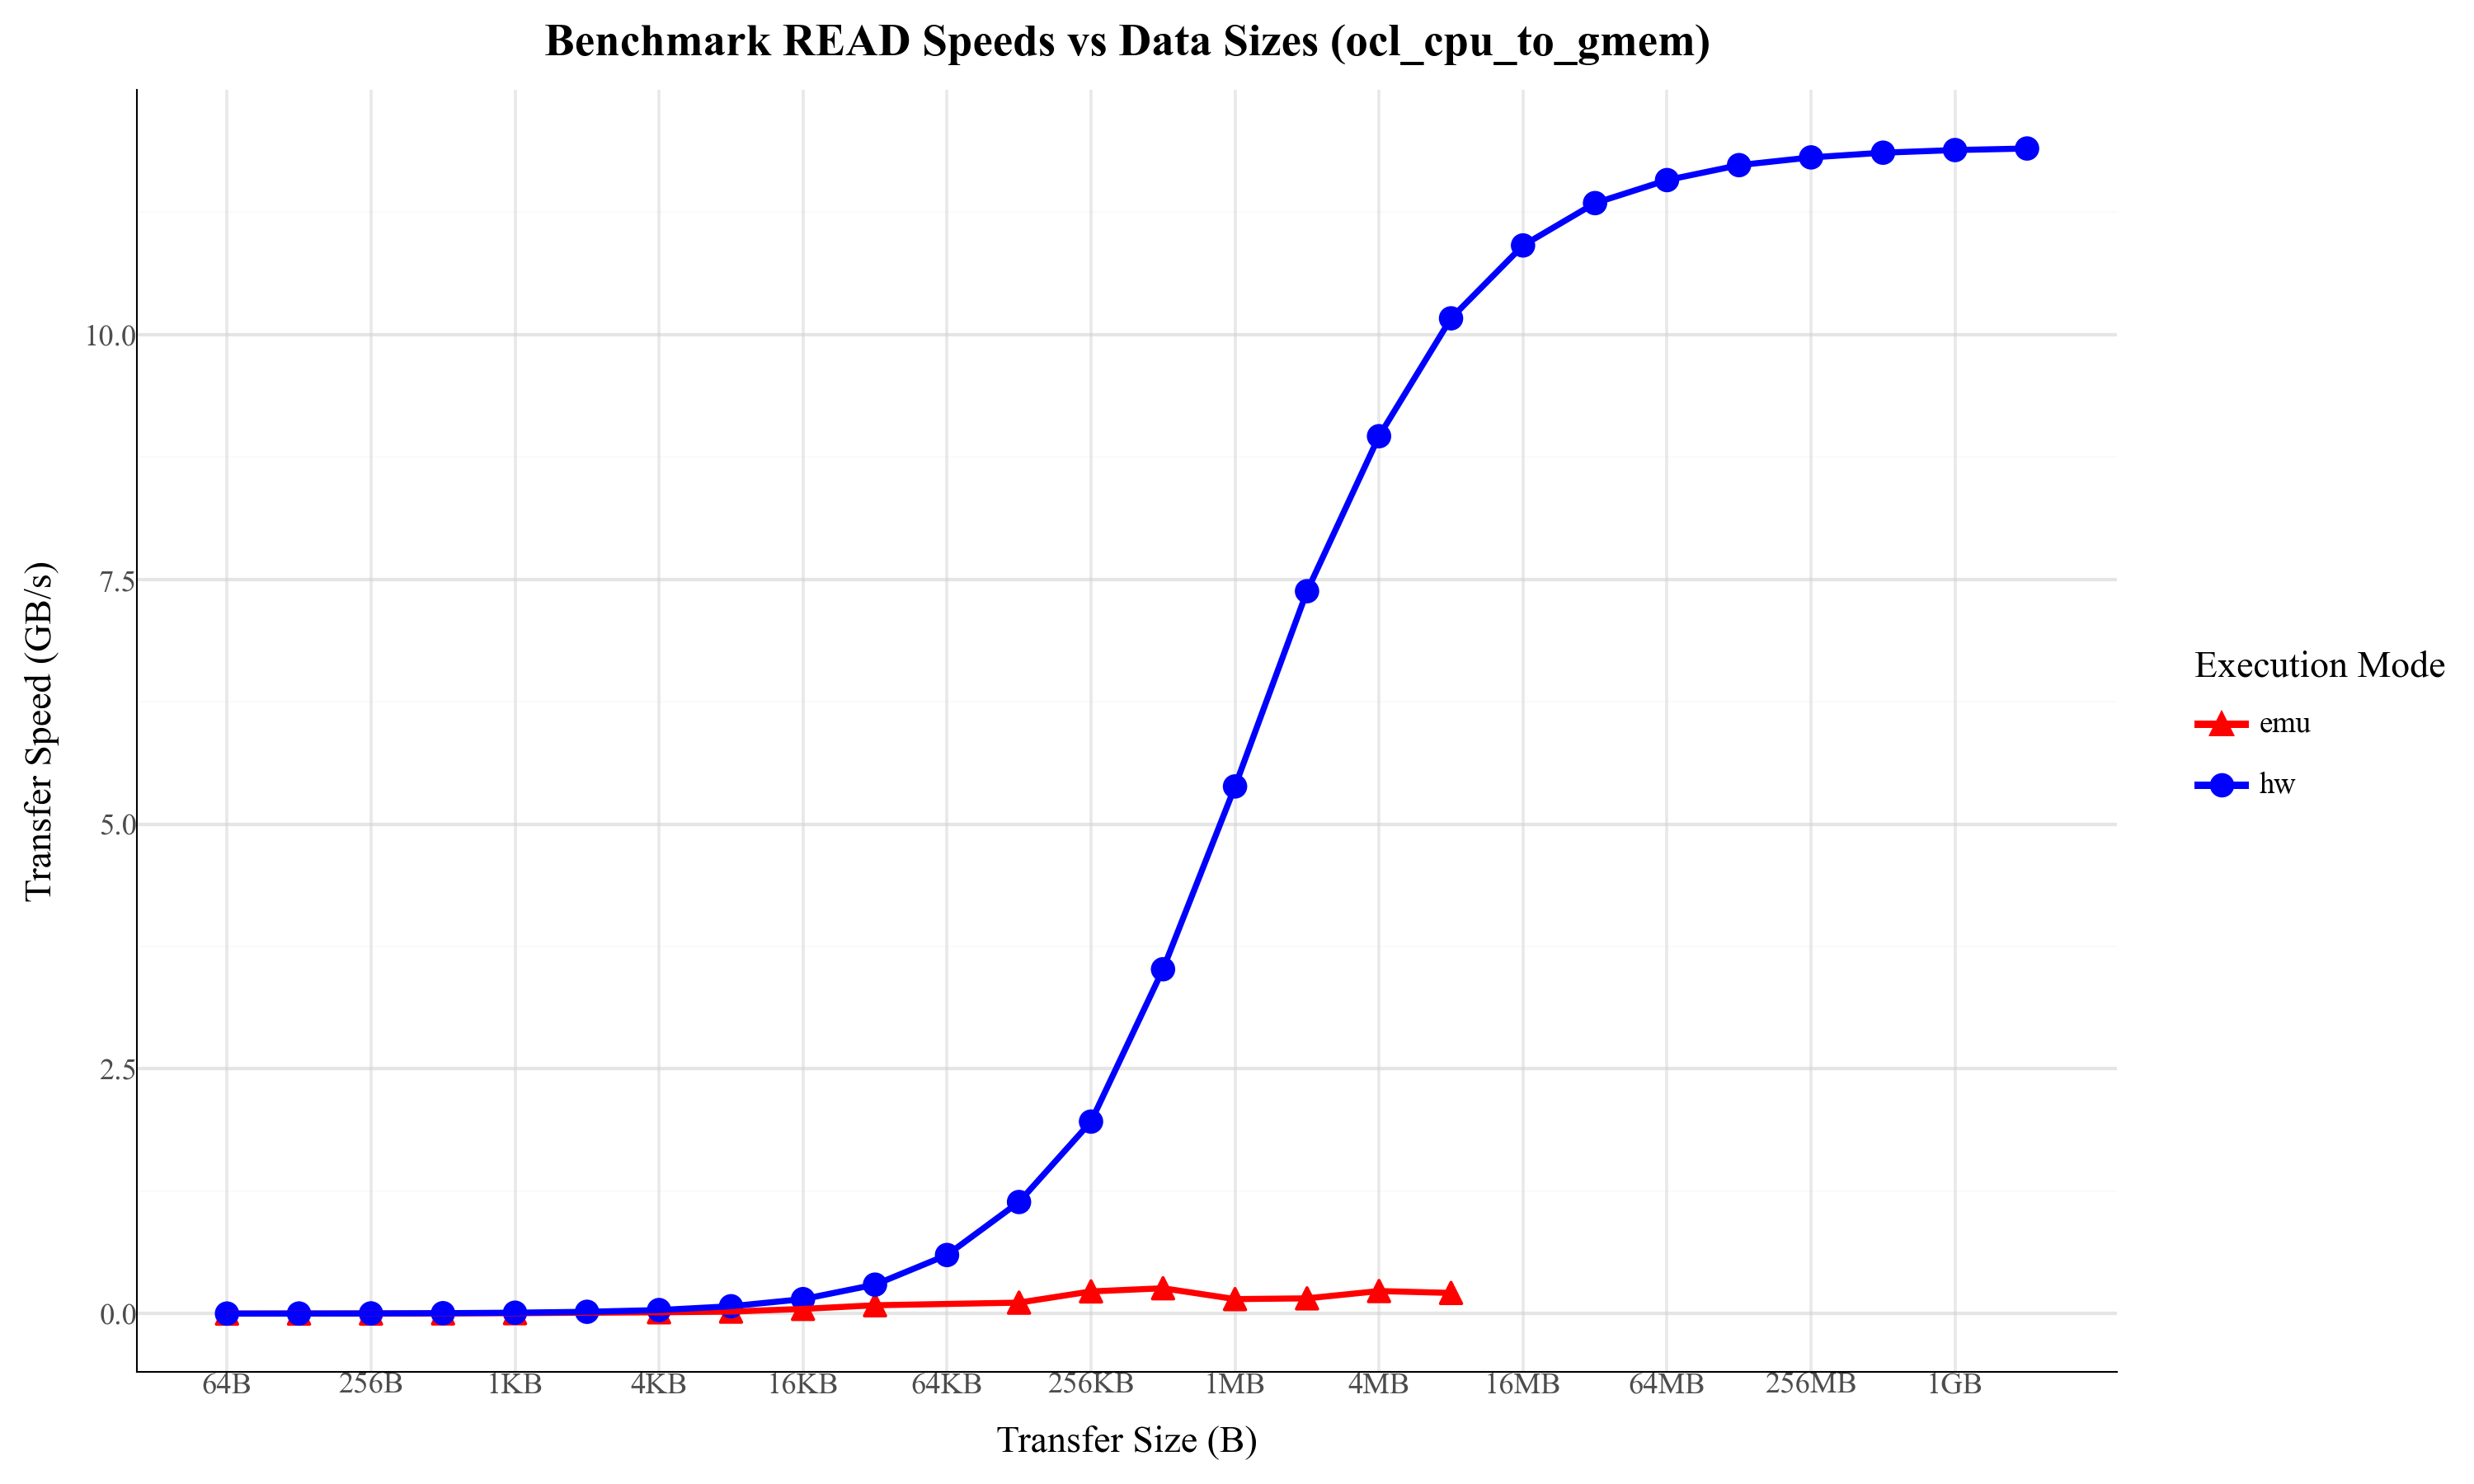
\includegraphics[width=0.9\linewidth]{content/ocl_cpu_to_gmem_READ.png}
    \caption{Log10 Graph of Data READ Speeds Comparison from CPU to GMEM for HW and EMU using OCL.}
    \label{fig:enter-label}
\end{figure}

\begin{figure}[H]
    \centering
    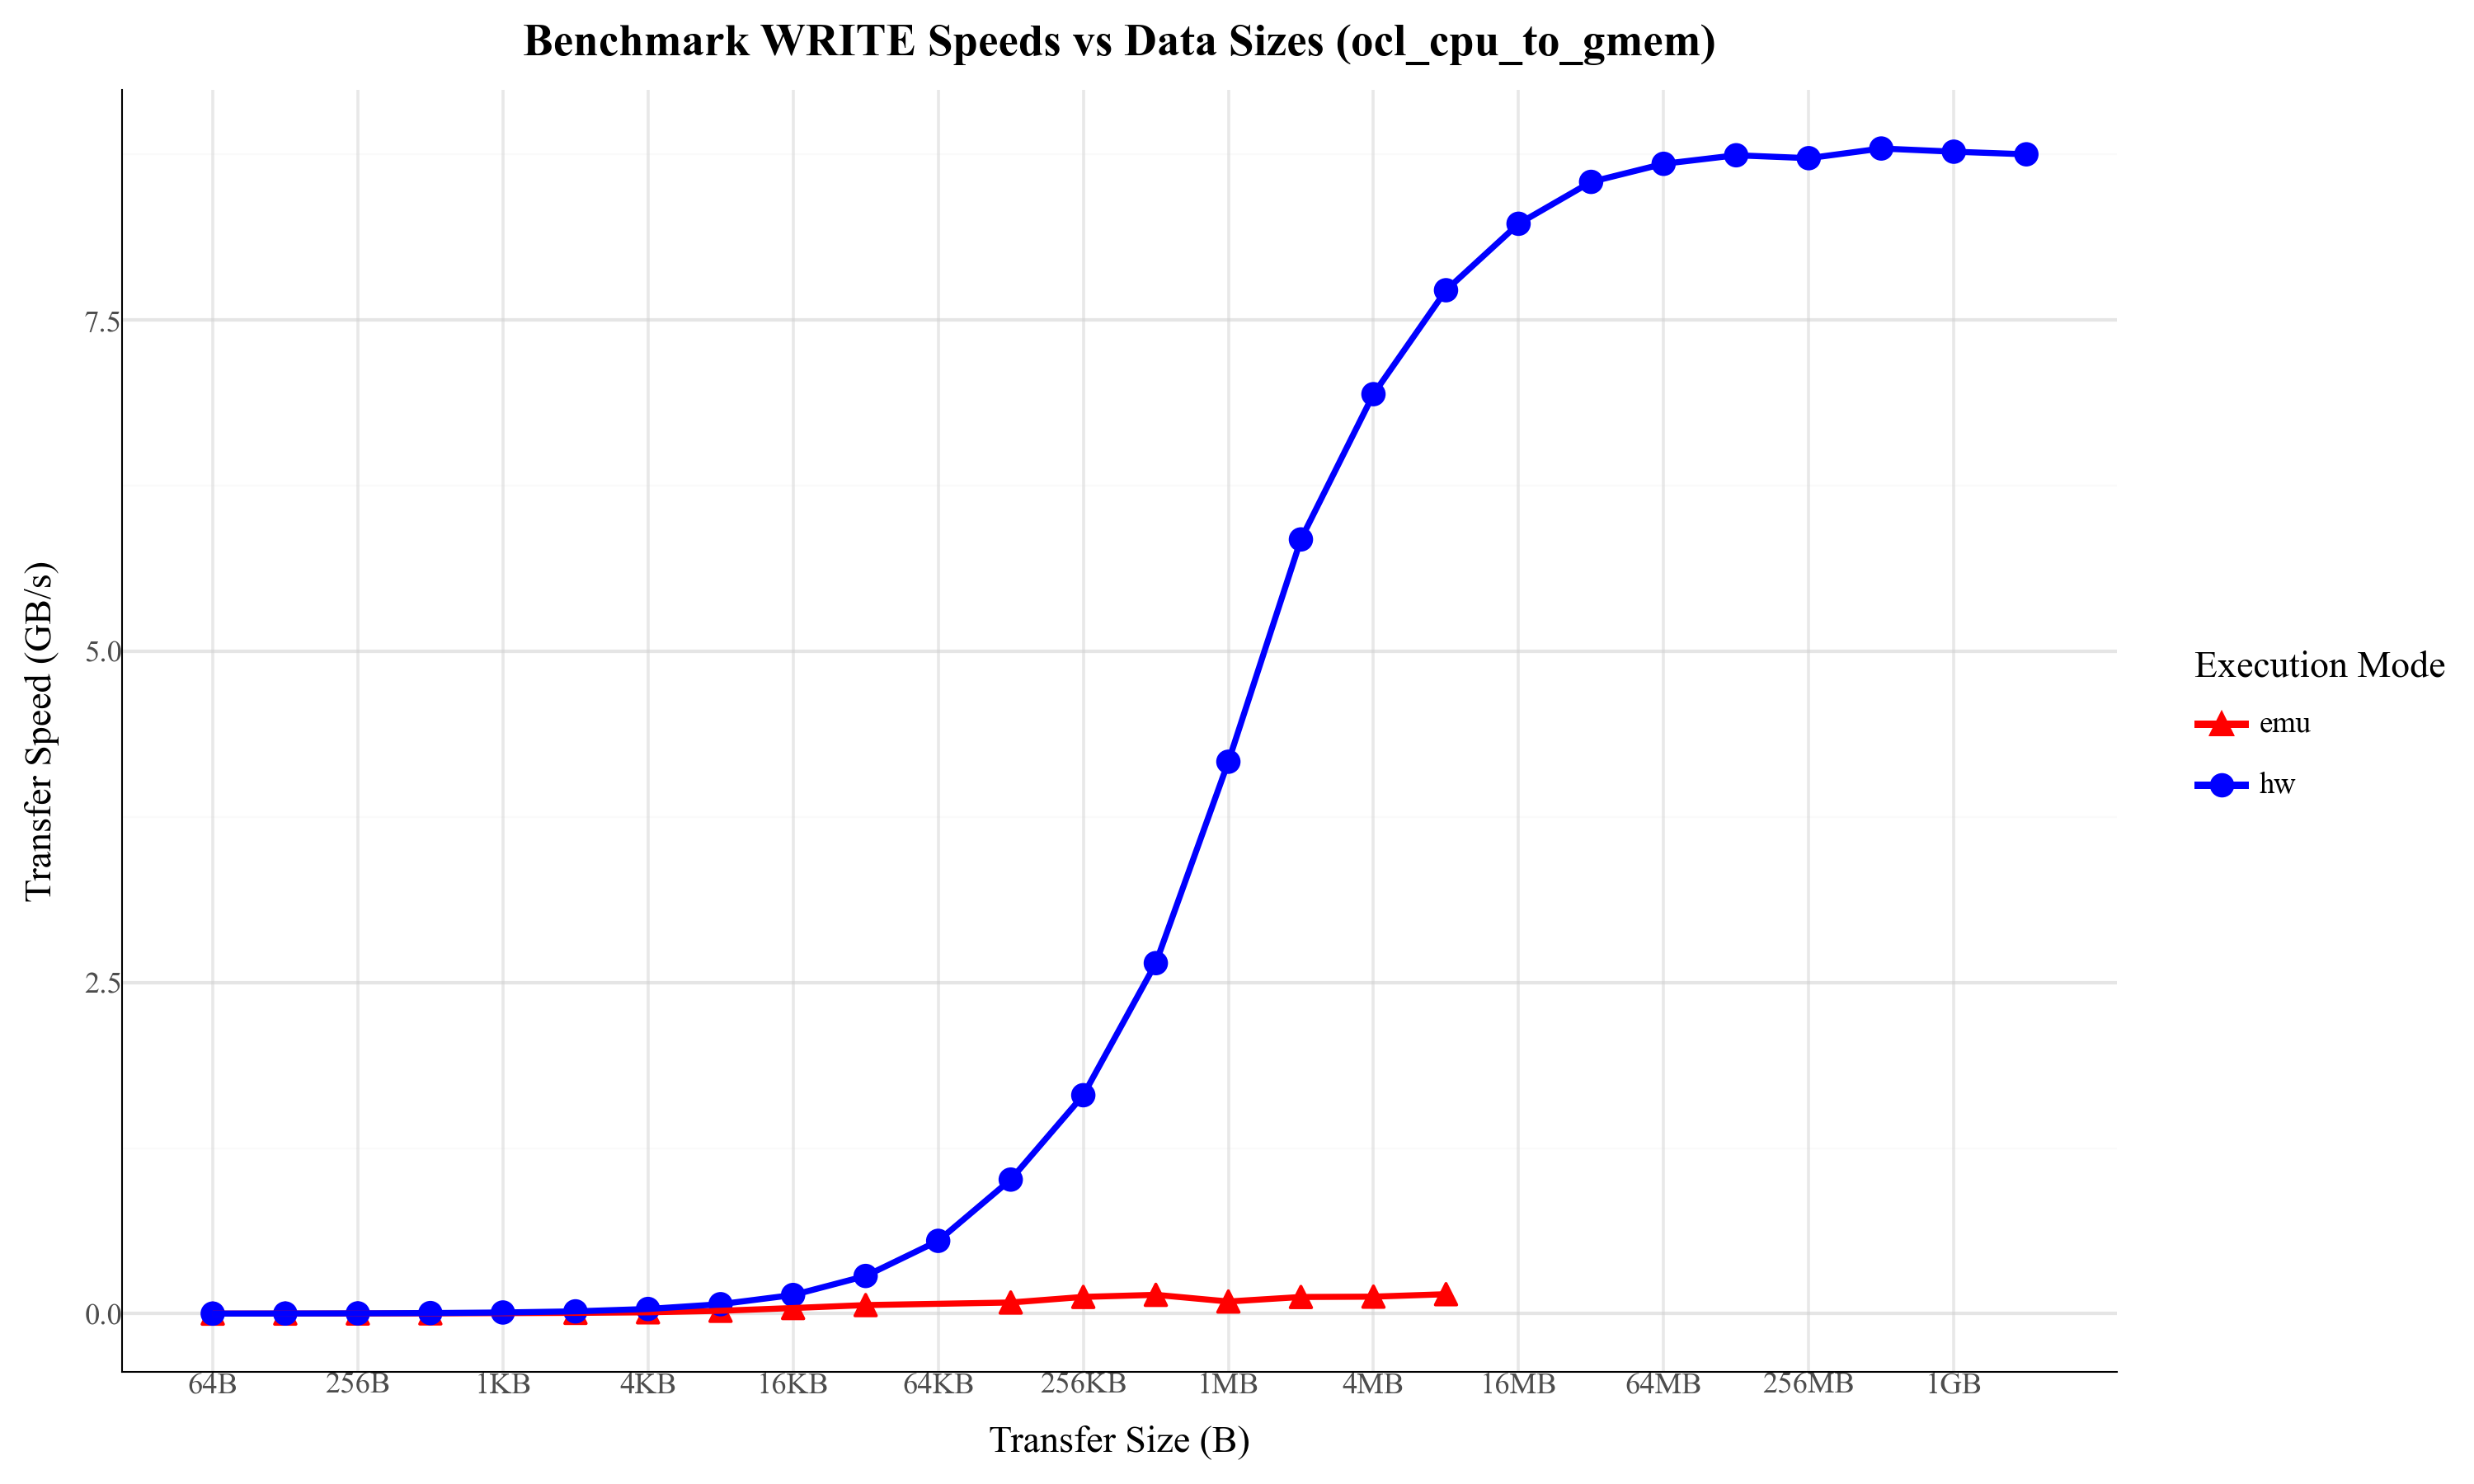
\includegraphics[width=0.9\linewidth]{content/ocl_cpu_to_gmem_WRITE.png}
    \caption{Log10 Graph of Data WRITE Speeds Comparison from CPU to GMEM for HW and EMU using OCL.}
    \label{fig:enter-label}
\end{figure}

\begin{figure}[H]
    \centering
    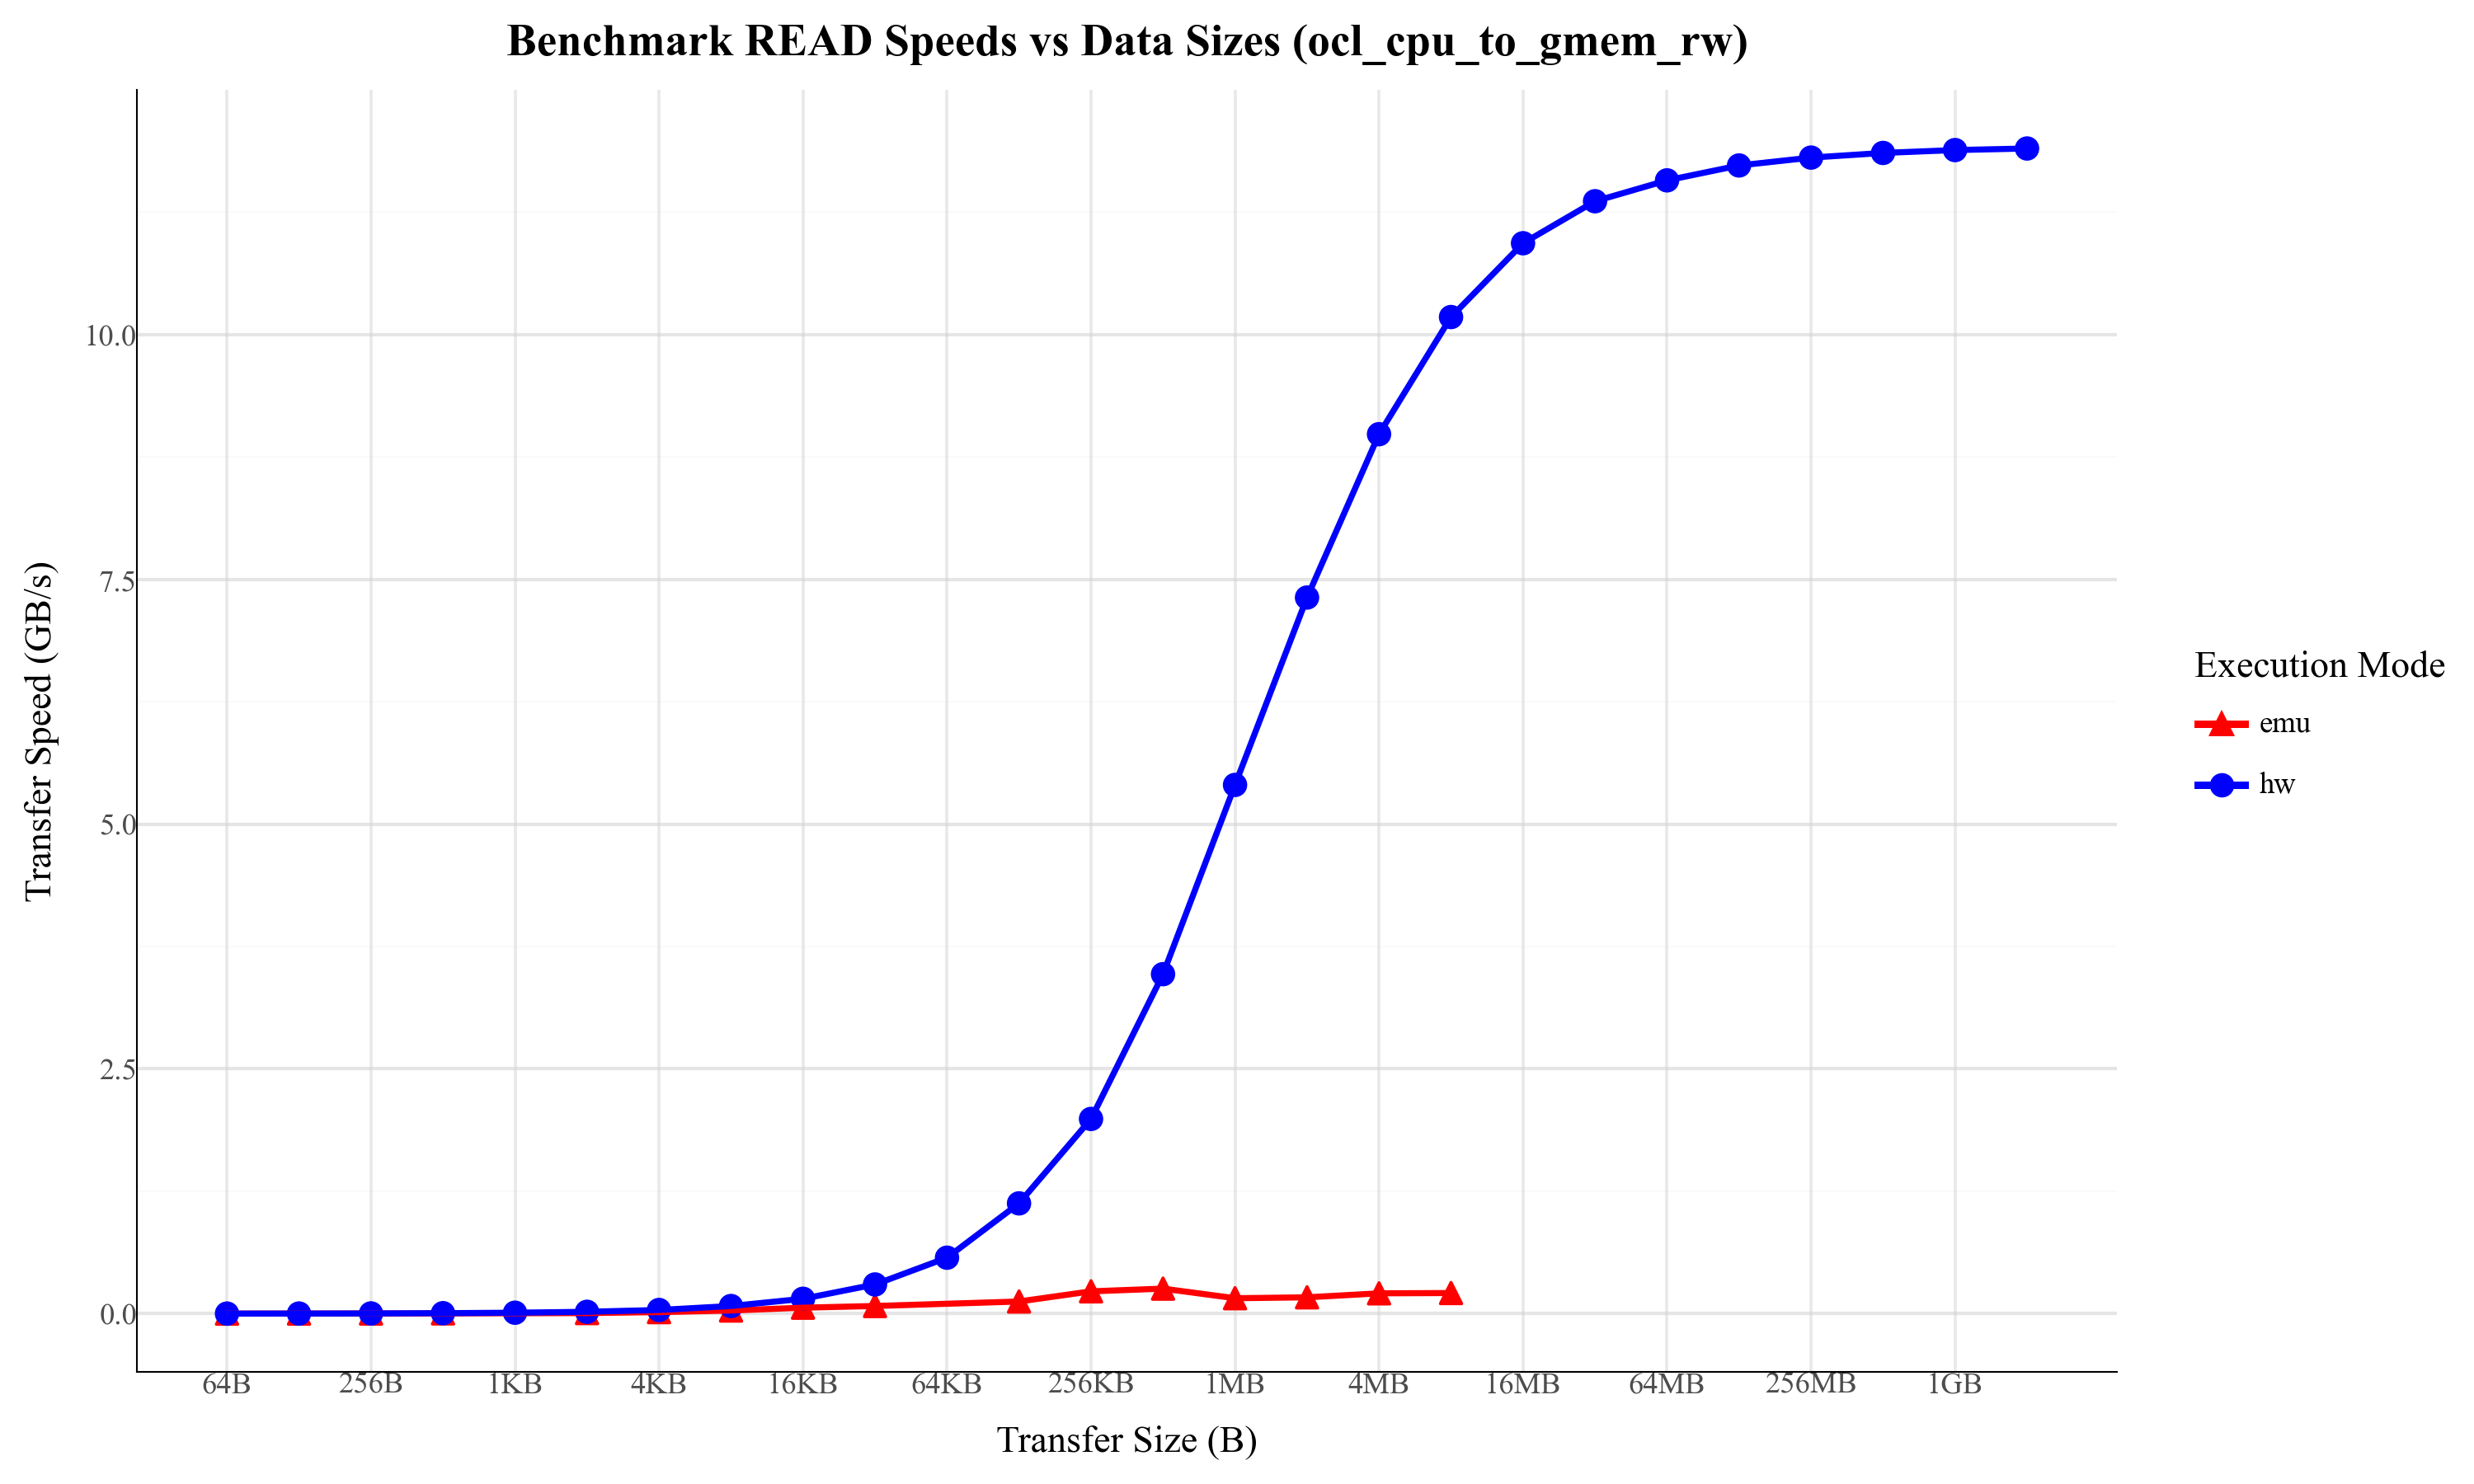
\includegraphics[width=0.9\linewidth]{content/ocl_cpu_to_gmem_rw_READ.png}
    \caption{Log10 Graph of Consecutive Data READ Speeds Comparison from CPU to GMEM for HW and EMU using OCL.}
    \label{fig:enter-label}
\end{figure}

\begin{figure}[H]
    \centering
    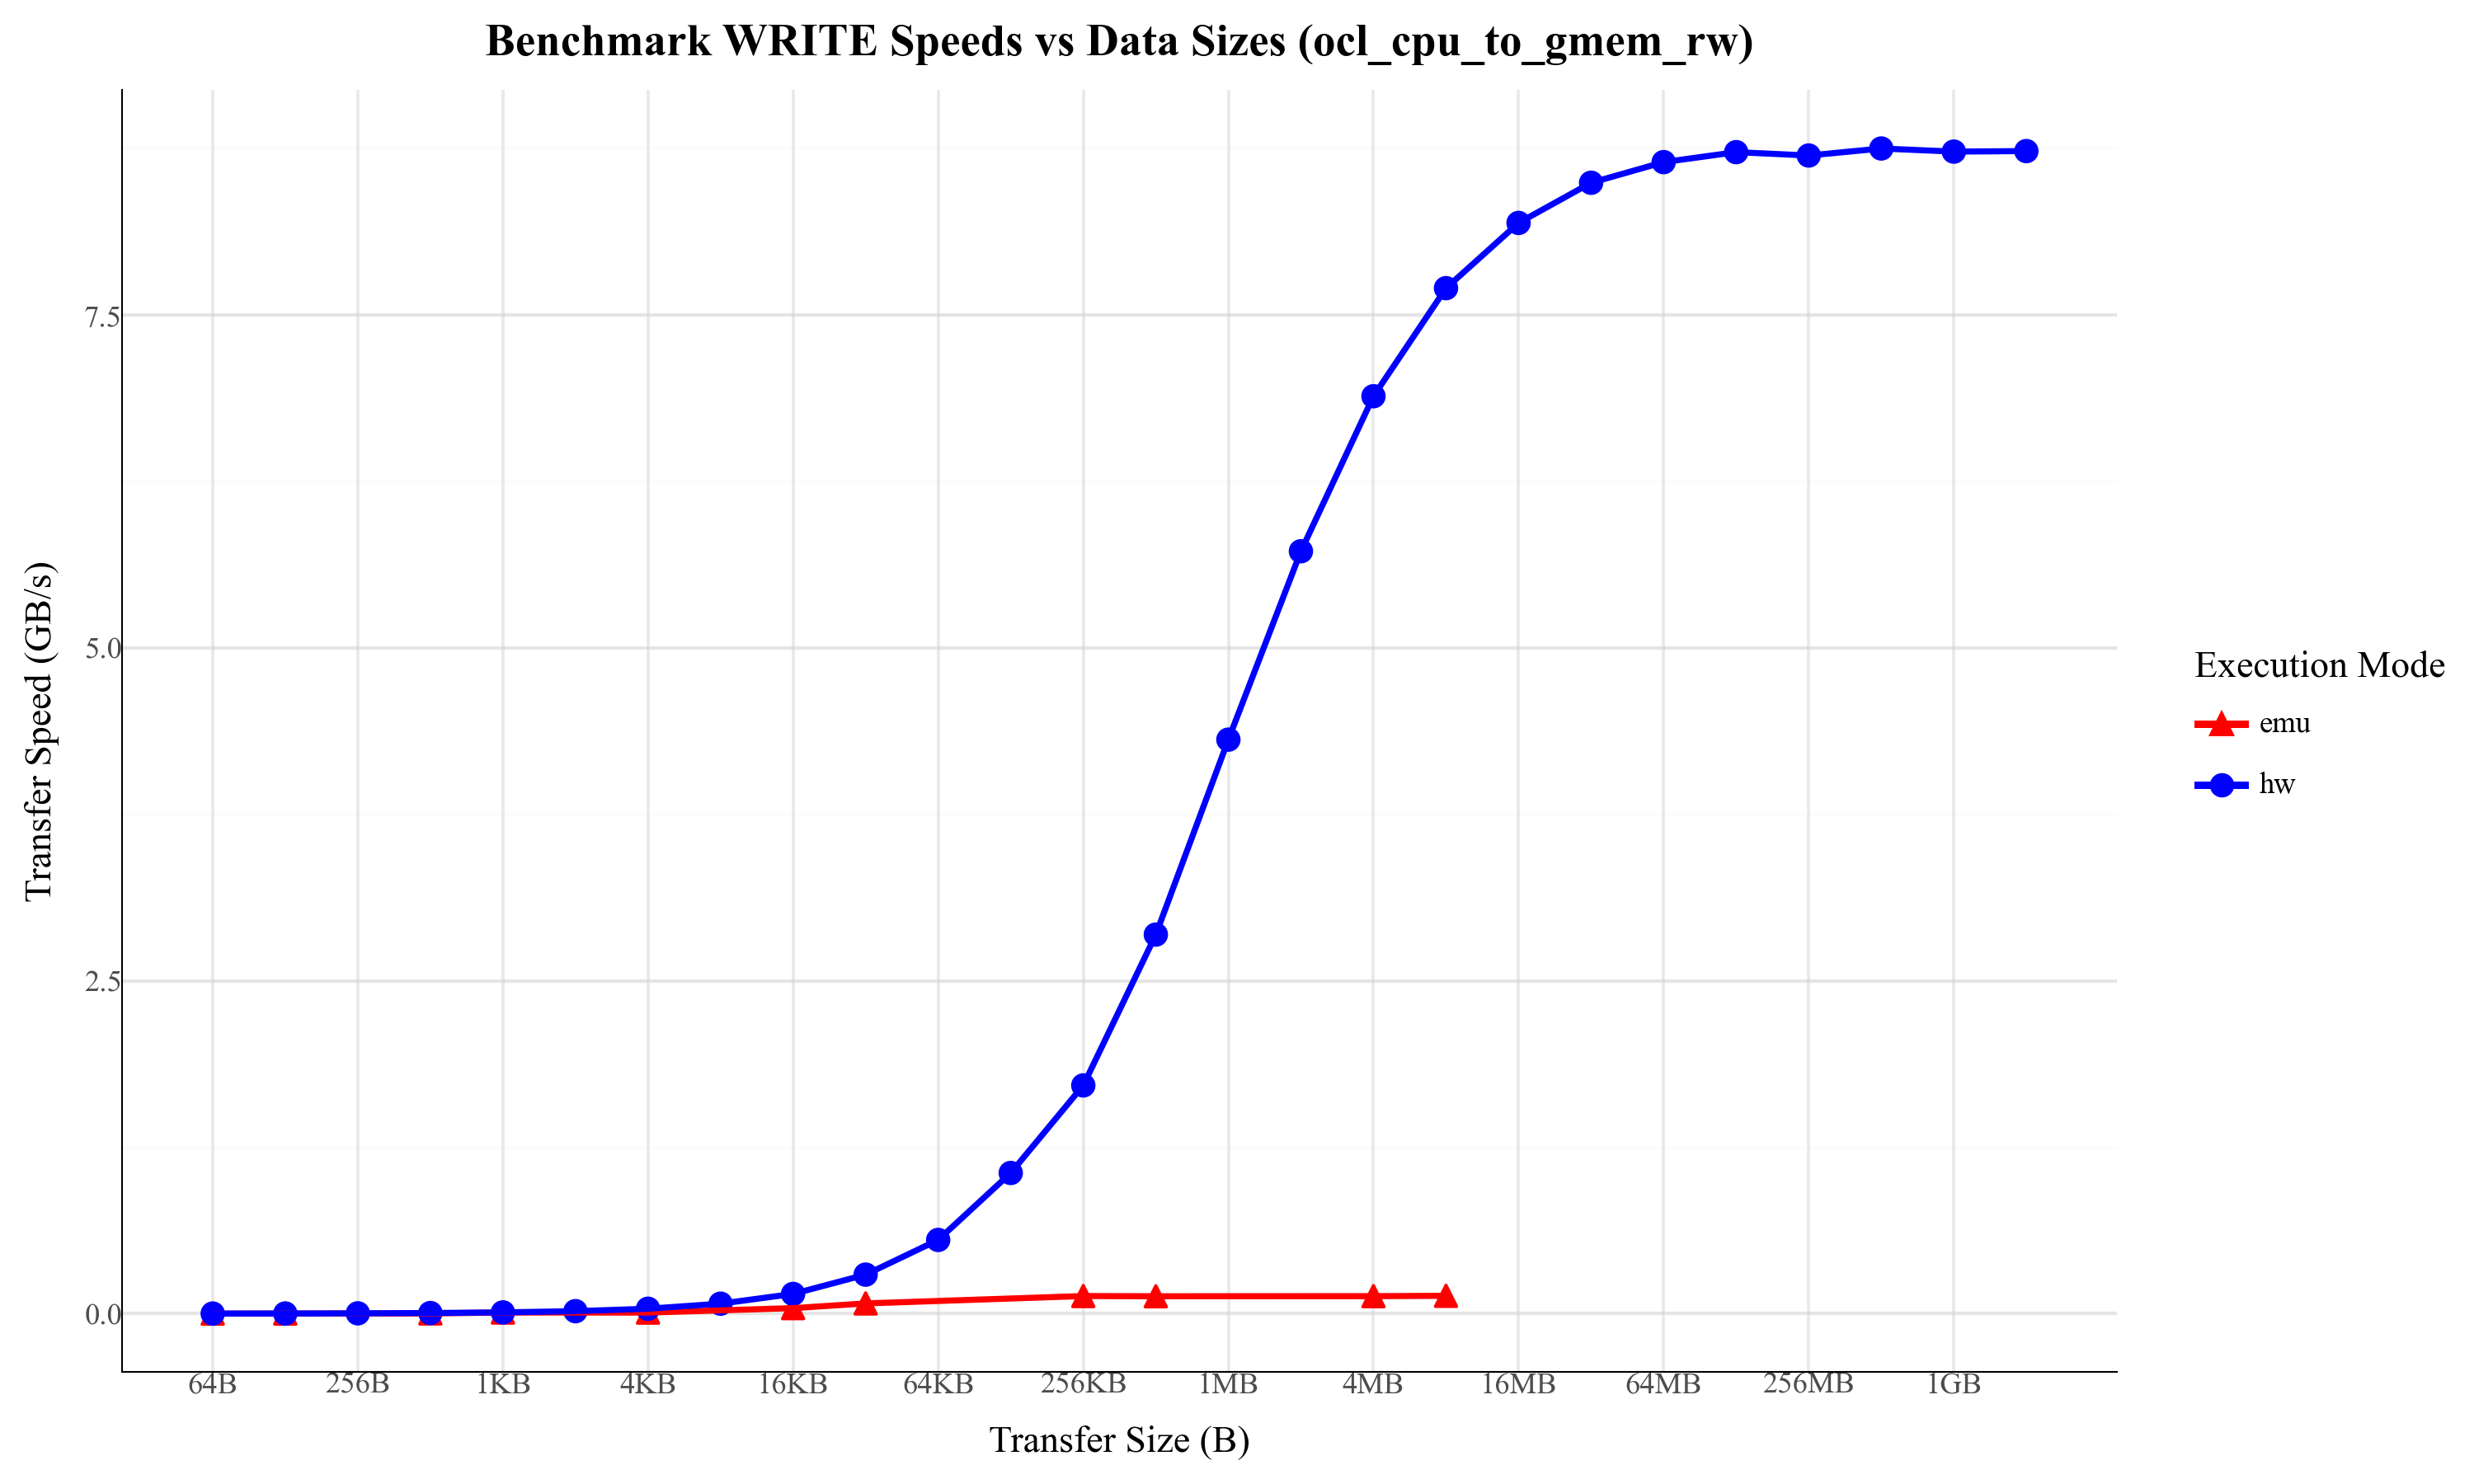
\includegraphics[width=0.9\linewidth]{content/ocl_cpu_to_gmem_rw_WRITE.png}
    \caption{Log10 Graph of Consecutive Data WRITE Speeds Comparison from CPU to GMEM for HW and EMU using OCL.}
    \label{fig:enter-label}
\end{figure}

\begin{figure}[H]
    \centering
    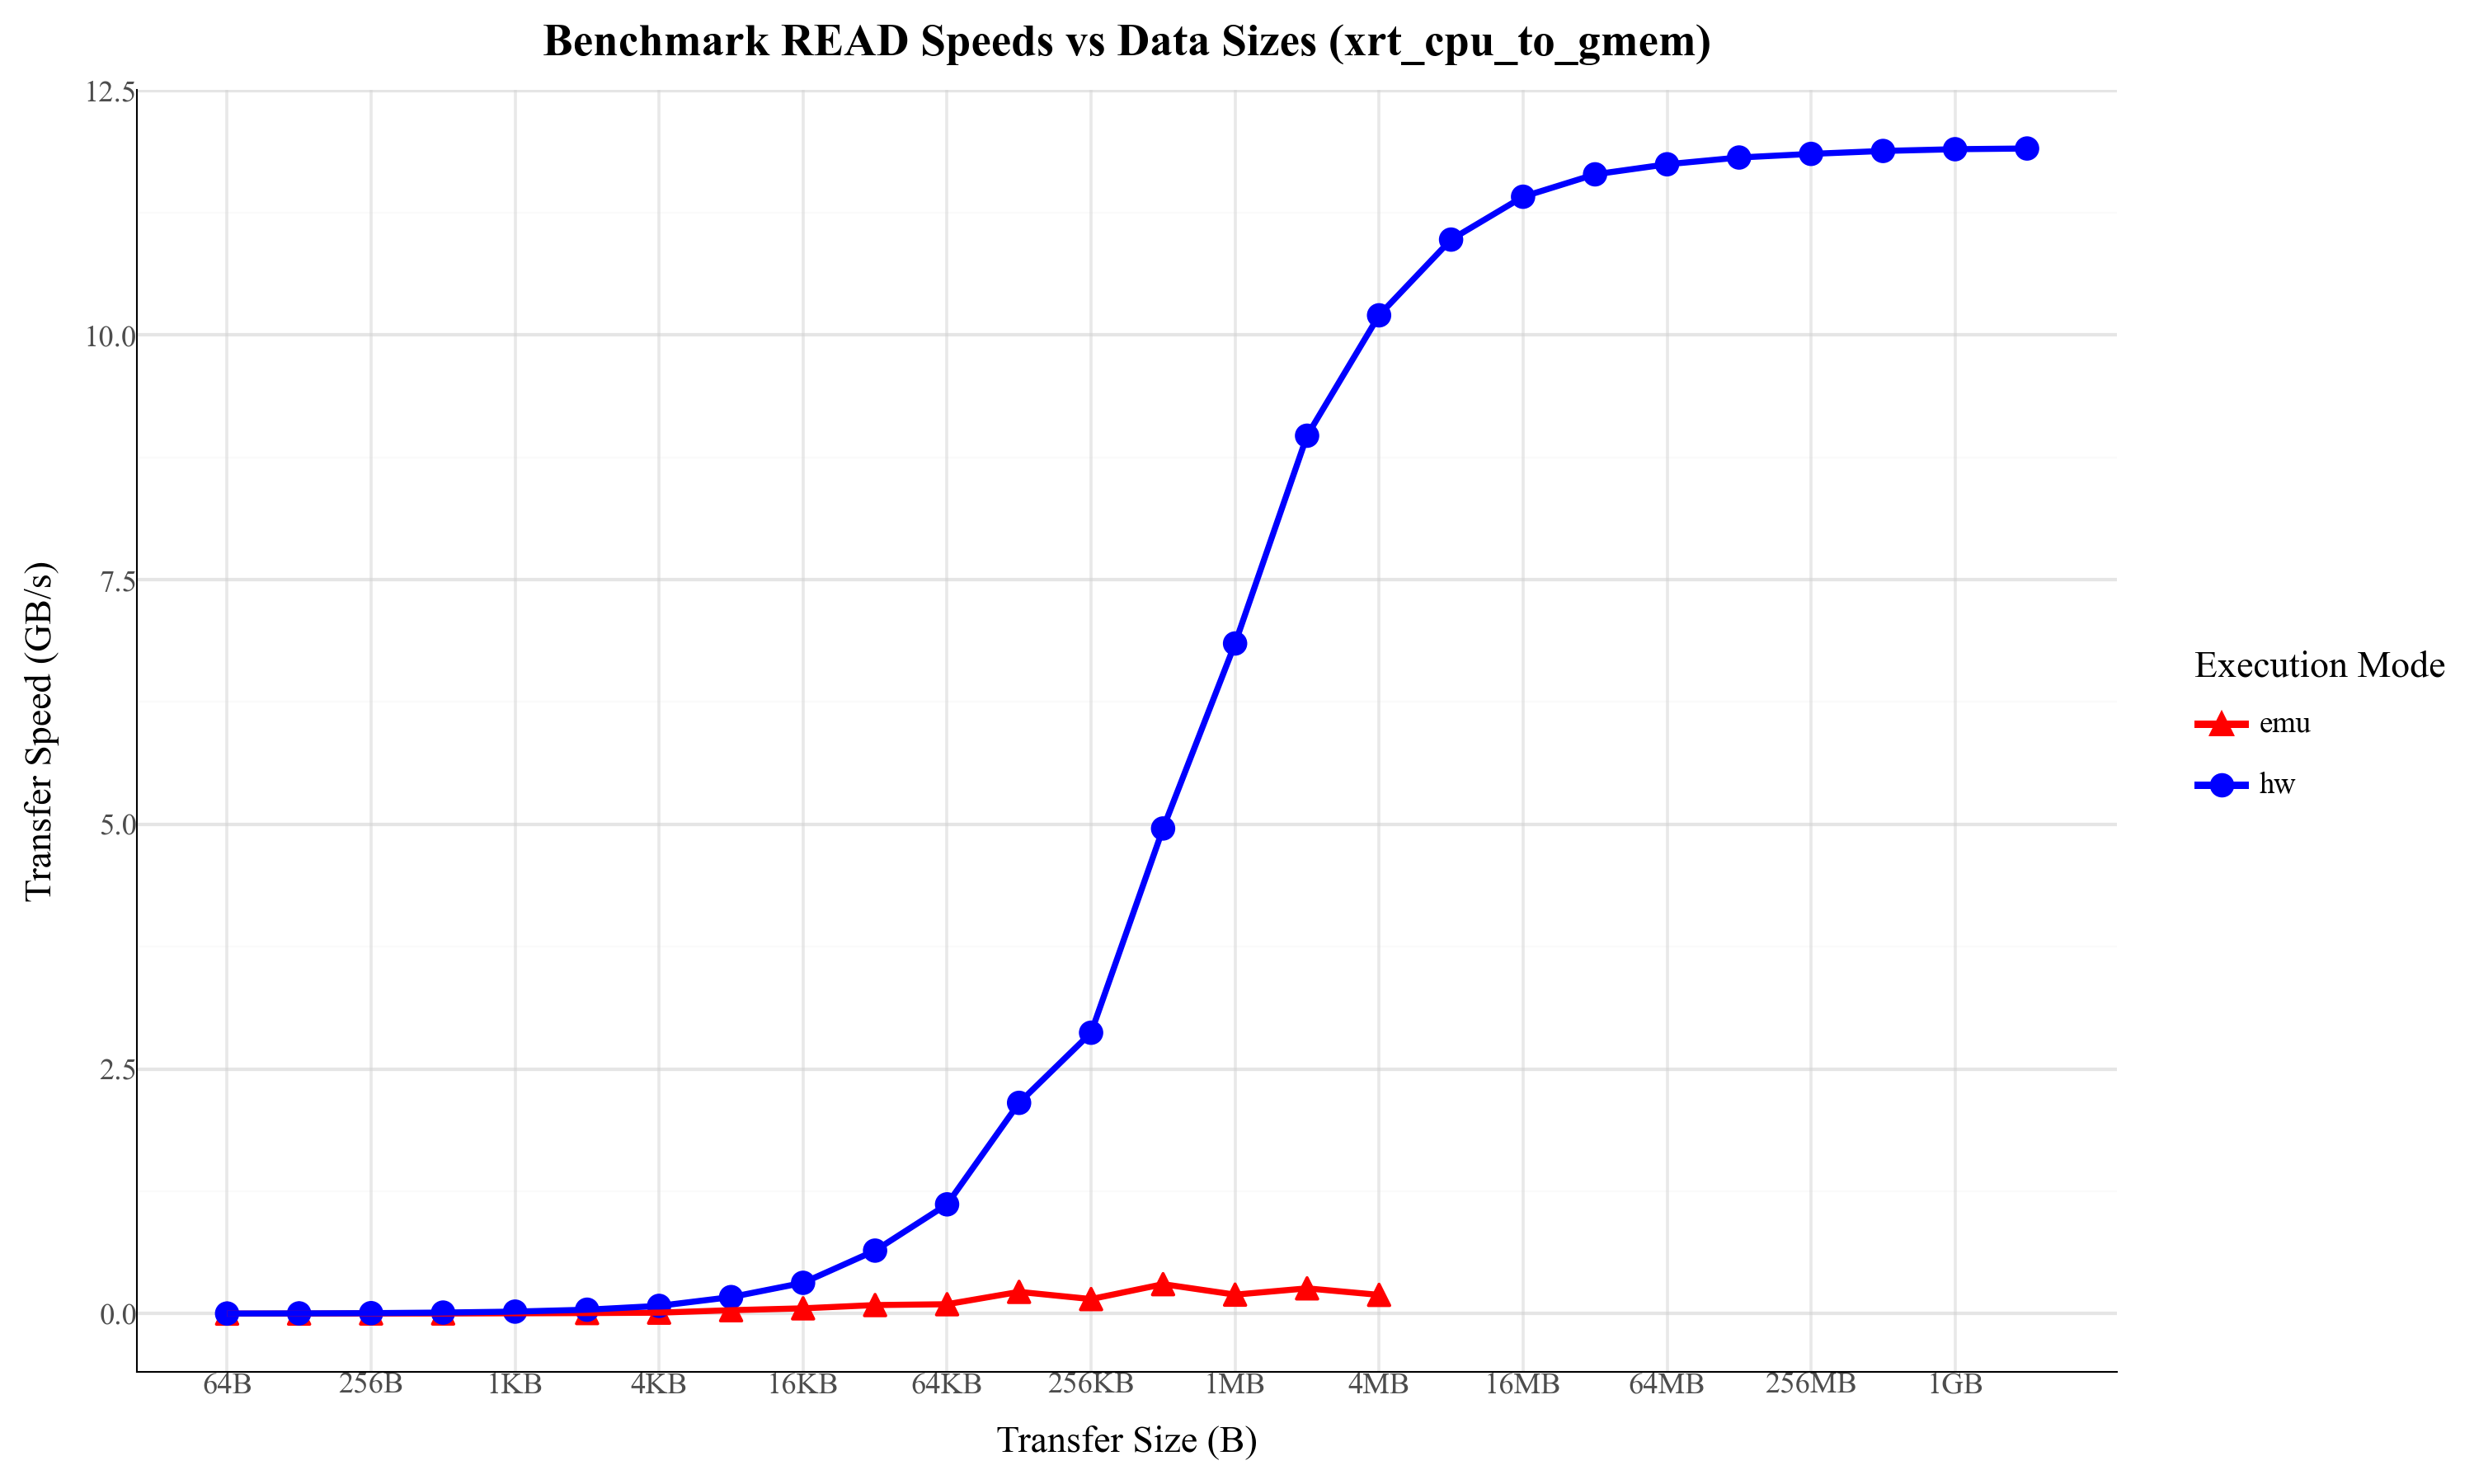
\includegraphics[width=0.9\linewidth]{content/xrt_cpu_to_gmem_READ.png}
    \caption{Log10 Graph of Data READ Speeds Comparison from CPU to GMEM for HW and EMU using XRT API.}
    \label{fig:enter-label}
\end{figure}

\begin{figure}[H]
    \centering
    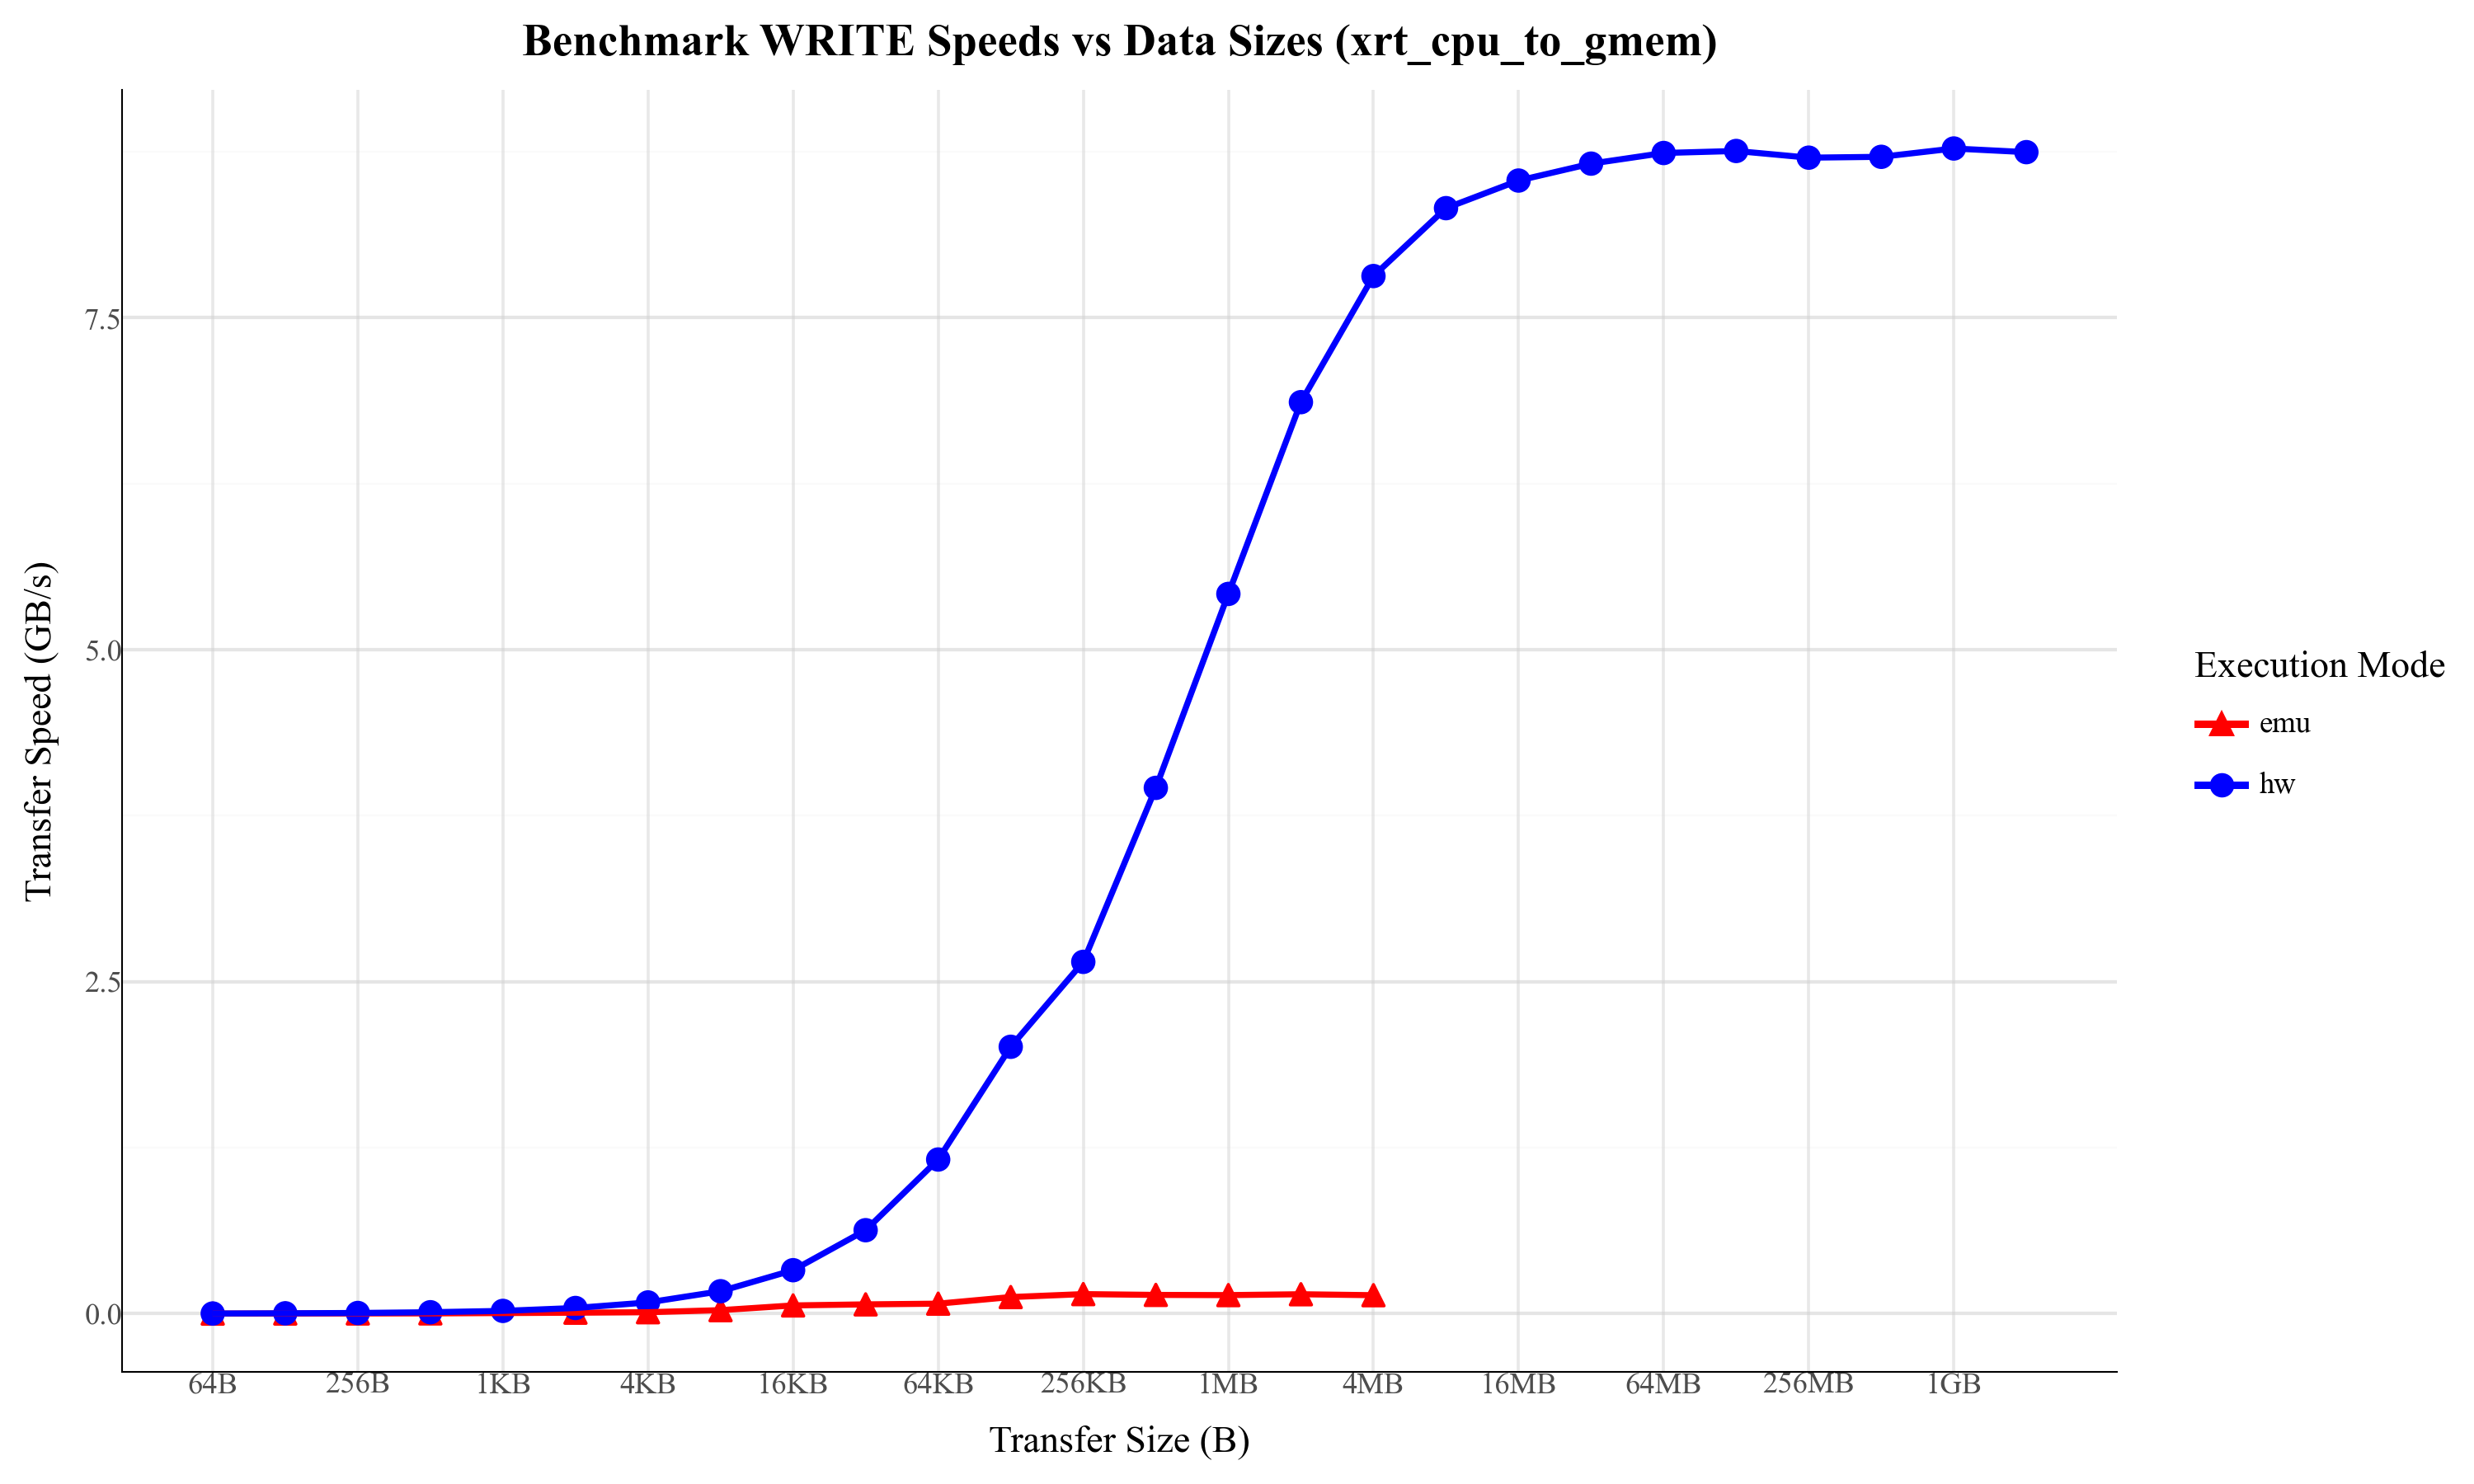
\includegraphics[width=0.9\linewidth]{content/xrt_cpu_to_gmem_WRITE.png}
    \caption{Log10 Graph of Data WRITE Speeds Comparison from CPU to GMEM for HW and EMU using XRT API.}
    \label{fig:enter-label}
\end{figure}

\begin{figure}[H]
    \centering
    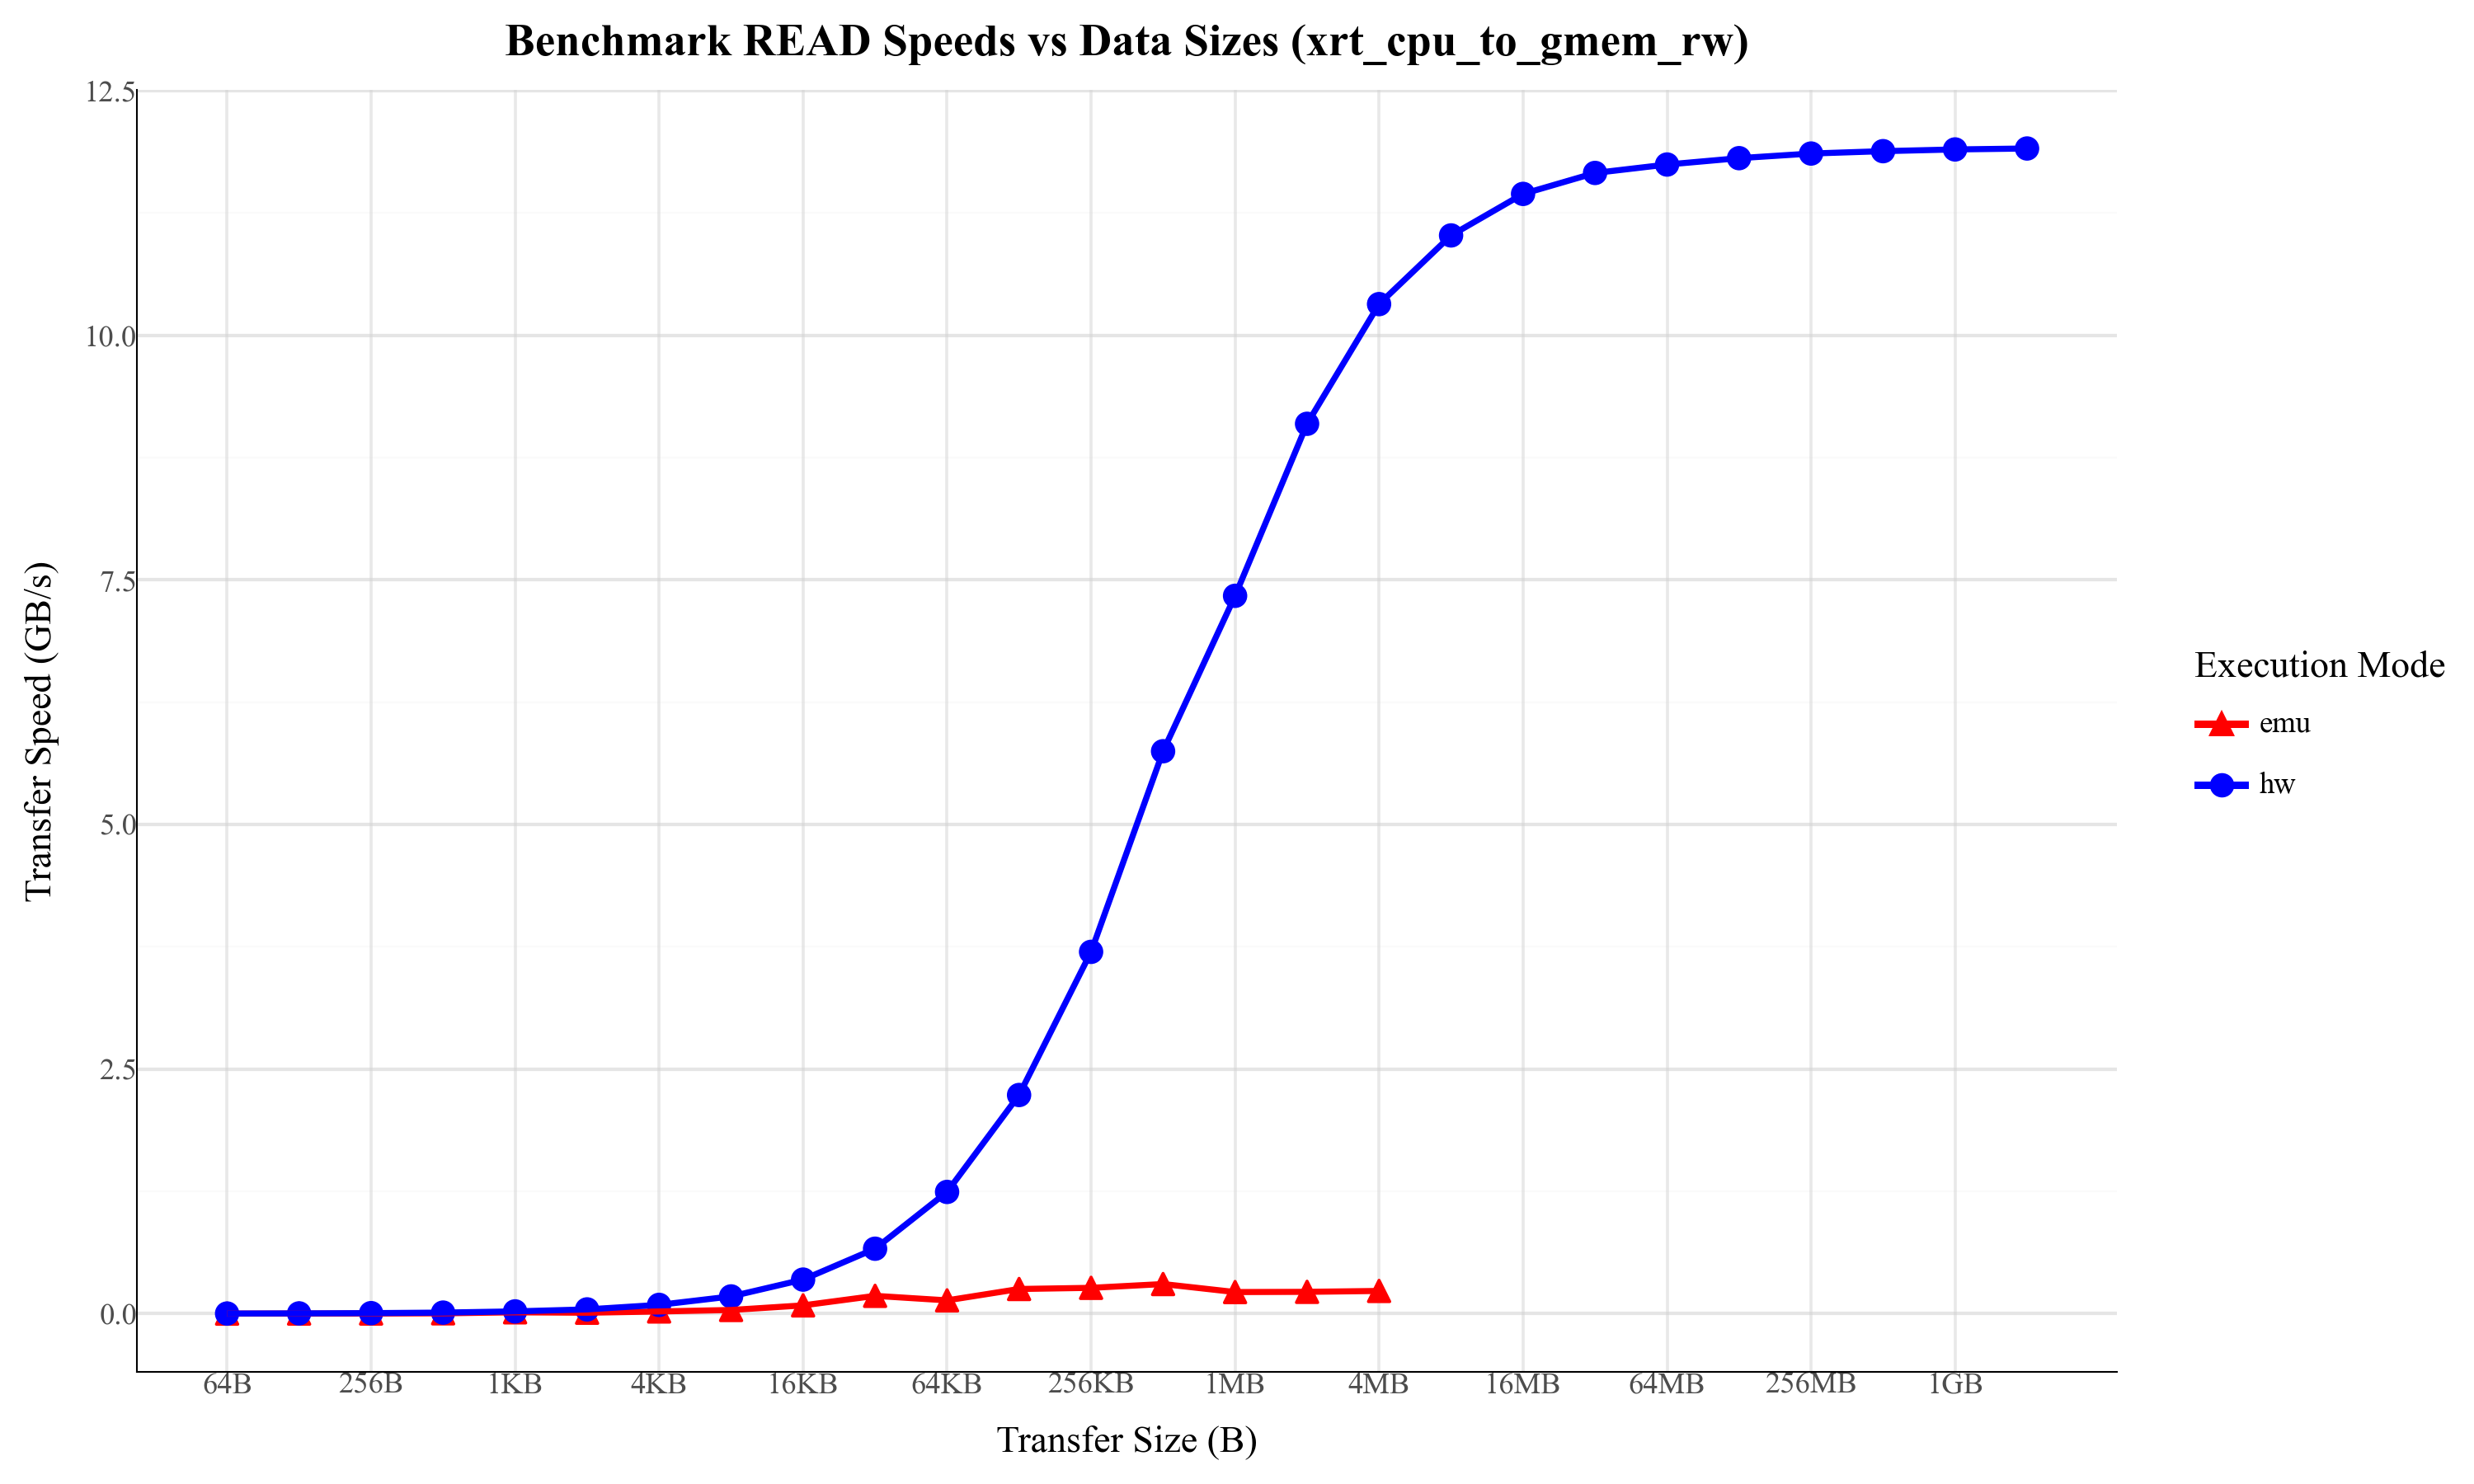
\includegraphics[width=0.9\linewidth]{content/xrt_cpu_to_gmem_rw_READ.png}
    \caption{Log10 Graph of Consecutive Data READ Speeds Comparison from CPU to GMEM for HW and EMU using XRT API.}
    \label{fig:enter-label}
\end{figure}

\begin{figure}[H]
    \centering
    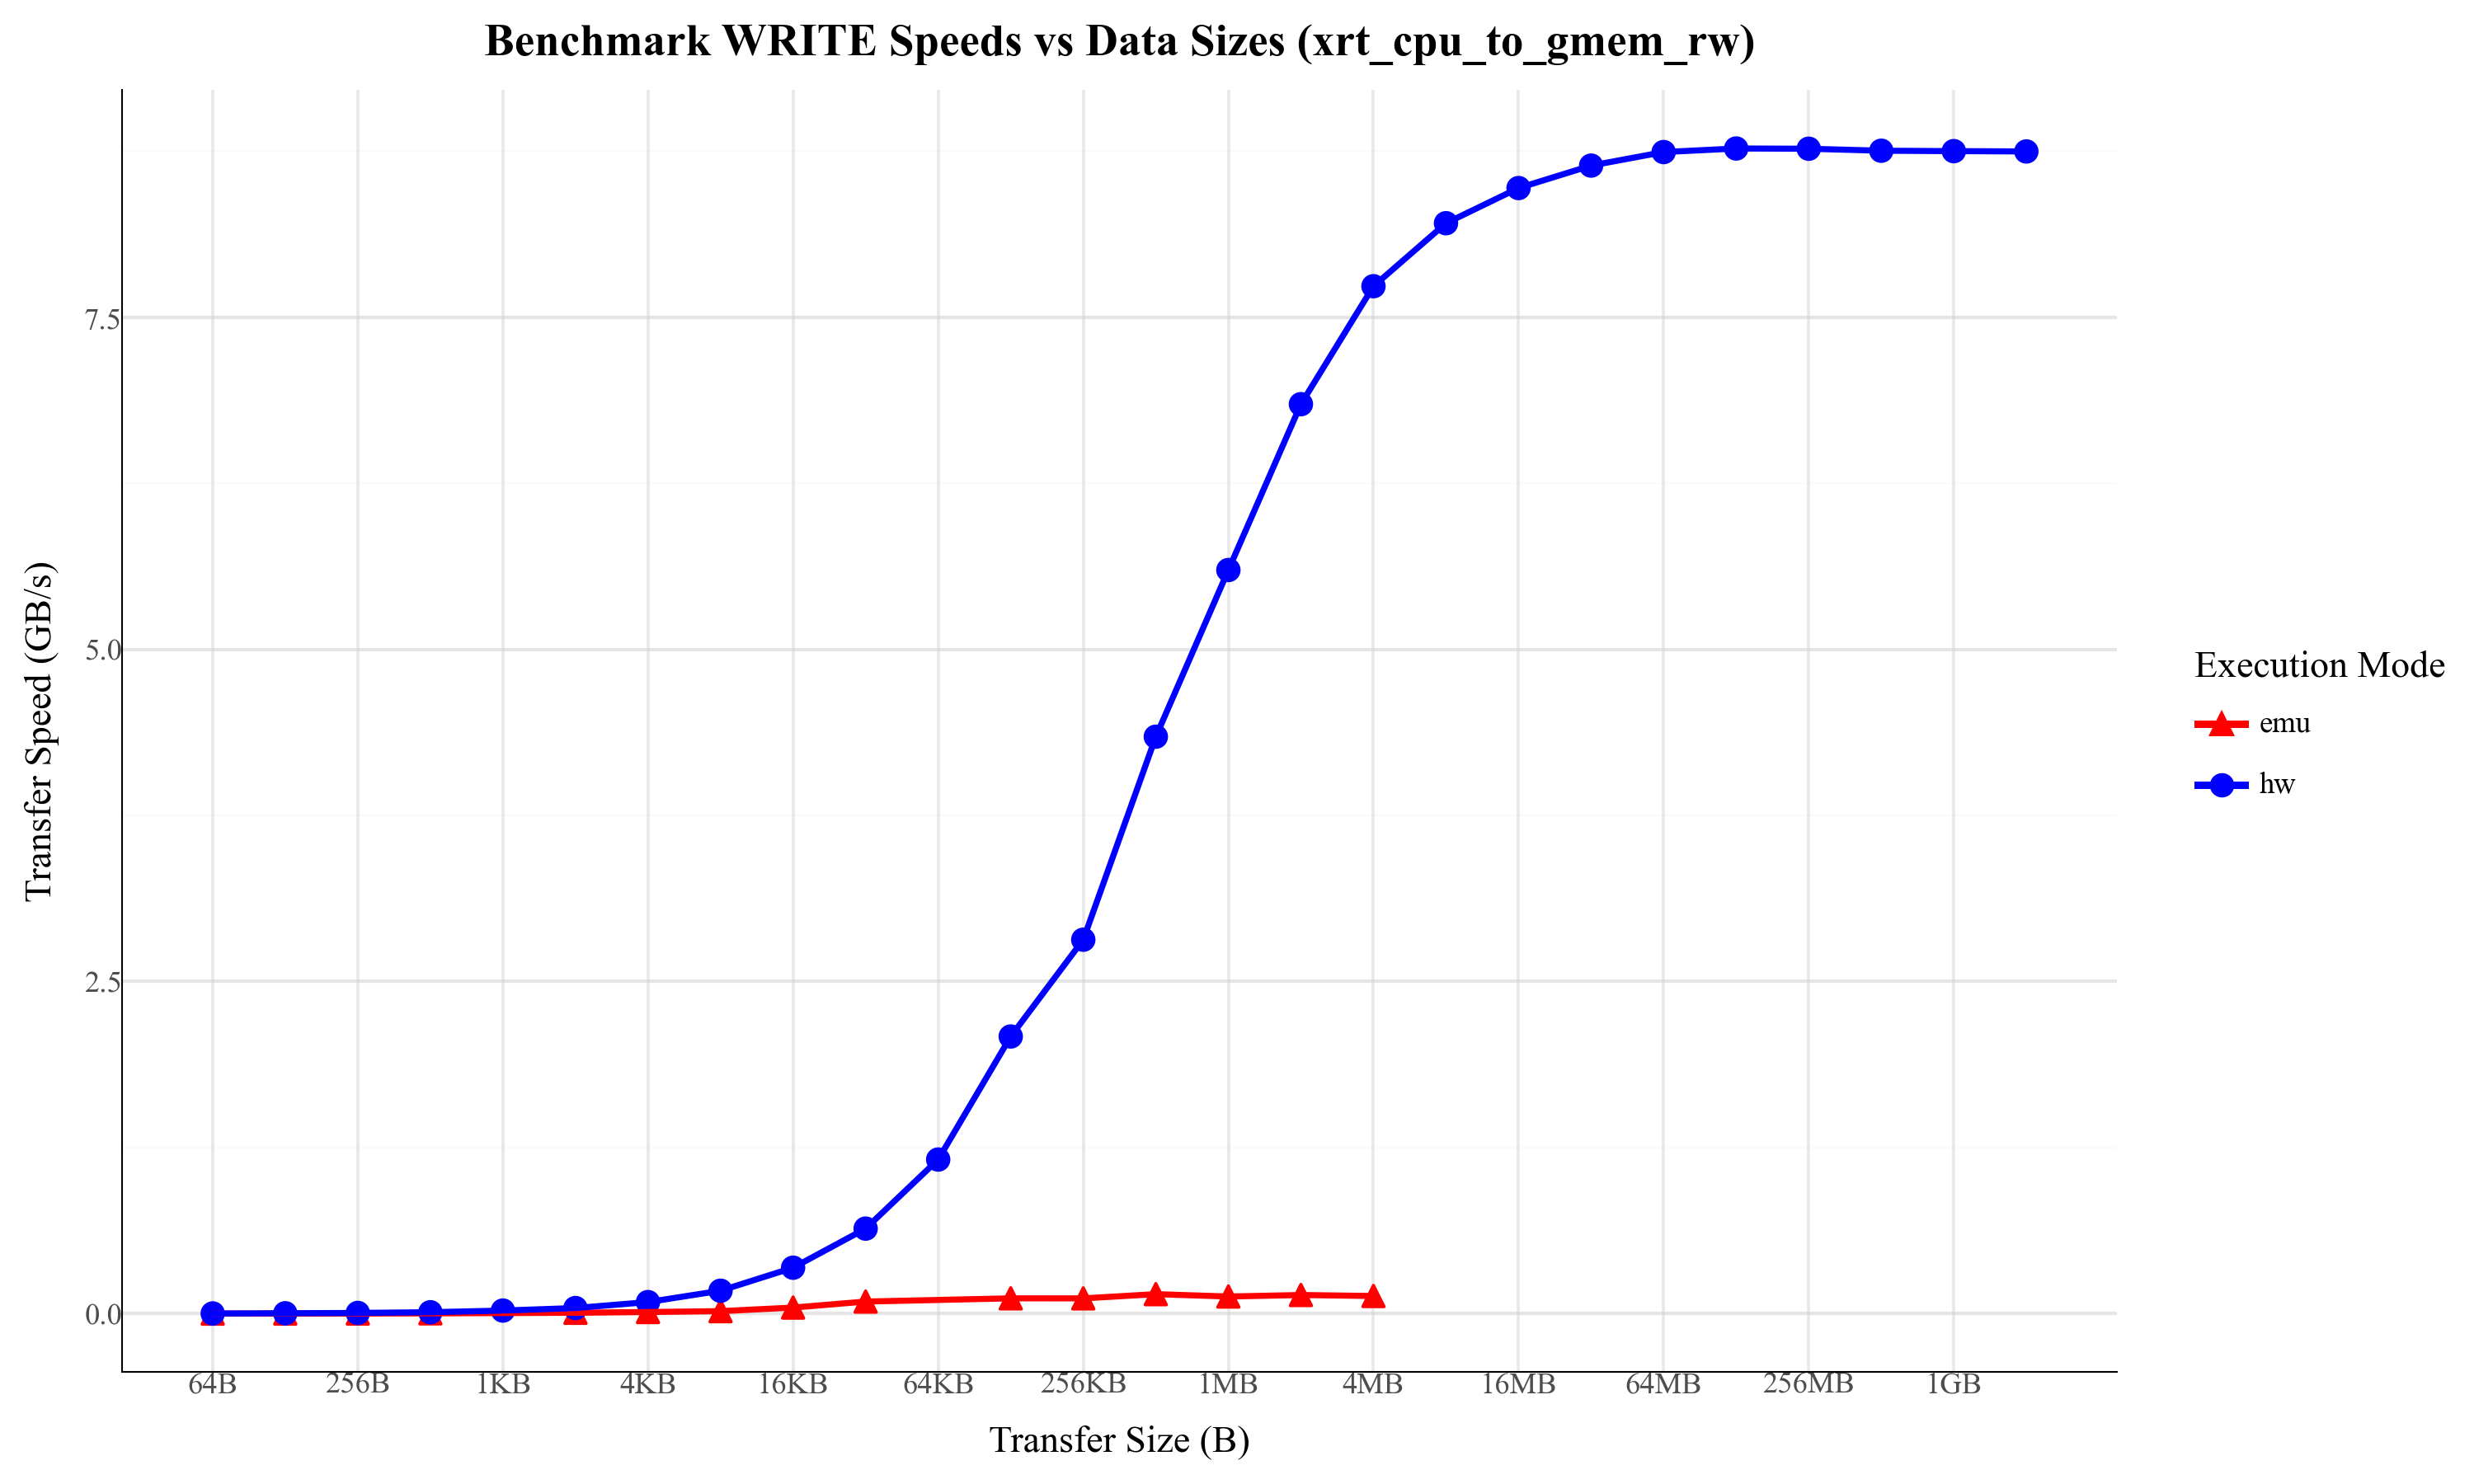
\includegraphics[width=0.9\linewidth]{content/xrt_cpu_to_gmem_rw_WRITE.png}
    \caption{Log10 Graph of Consecutive Data WRITE Speeds Comparison from CPU to GMEM for HW and EMU using XRT API.}
    \label{fig:enter-label}
\end{figure}

% Removed due to lacking support on HW.
% \begin{figure}[H]
%     \centering
%     \includegraphics[width=1.0\linewidth]{content/ocl_fpga_to_gmem_READ.png}
%     \caption{Log10 Graph of Data READ Speeds Comparison from FPGA to GMEM for HW (unsupported) and EMU.}
%     \label{fig:enter-label}
% \end{figure}

% \begin{figure}[H]
%     \centering
%     \includegraphics[width=1.0\linewidth]{content/ocl_fpga_to_gmem_WRITE.png}
%     \caption{Log10 Graph of Data WRITE Speeds Comparison from FPGA to GMEM for HW (unsupported) and EMU.}
%     \label{fig:enter-label}
% \end{figure}